\chapter{Vortex Methods}
\label{ch:vm}

Vortex Methods are a class of methods
used for direct numerical simulations
of incompressible viscous flows at high Reynold numbers~\cite{cottet00}.
In this chapter, the 2-D Vortex Blob Method is introduced,
along with its algorithmic characteristics.

\section{The mathematics of vorticity}
\label{sec:eqs-vort}

The vorticity field \(\mathbold\vort\)
of a fluid flow with velocity field~\(\vel = (u, v, w)\)
is defined as:%
\begin{equation}
  \label{eq:vorticity}
  \mathbold\vort = \curl\vel.
\end{equation}

Incompressible fluids are those for which
the volume of fluid elements remains constant in time.
This condition is described mathematically as~\(\nabla\cdot\vel = 0\).
It follows from the definition of vorticity that also~\(\nabla\cdot\mathbold\vort = 0\).

The vorticity is orthogonal to the velocity on every point of the fluid.
Therefore, in a two-dimensional flow,
the only non-zero component of the vorticity is the \(z\) component. 
It this case, it is customary to consider the vorticity as a scalar field
\(\vort = v_x - u_y\)\footnotemark,
such that \(\mathbold\vort = \vort\hat{\vec k}\).

\footnotetext{Unless otherwise stated, subindices represent partial derivatives.}

The motion of an incompressible fluid
is governed by the conservations laws of mass and momentum.
These laws are typically presented in an Eulerian reference frame,
where the equations are developed from the local analysis of the flow
in a fixed location in space, and are respectively:
\begin{align}
  \rho_t + \divergence(\rho\vel) &= 0, \\
  \rho(\vel_t + \vel\cdot\nabla\vel) &= -\nabla p + \mu\lapl\vel;
\end{align}
where \(\rho\) and \(p\) are the density and the pressure fields,
and \(\mu\) is the dynamic viscosity of the fluid.
These equations are also known respectively as
the continuity equation and the Navier-Stokes equation.

Vortex Methods, on the other hand, are based on the Lagrangian reference frame,
which views the fluid as a collection of fluid elements
that are freely translating, rotating and deforming,
while carrying the dependent quantities of the flow field,
such as velocity and temperature.
A full description of the flow is obtained by
identifying the initial location of the fluid elements
and the initial value of the dependent variable.

Both reference frames are conveniently related
by the material derivative operator \(D/Dt\),
defined as:
\begin{equation}
  \frac{D}{Dt} = \frac{\partial}{\partial t} + (\vel\cdot\nabla),
\end{equation}
which accounts for the rate change of a quantity along the flow trajectories.

The laws of conservation of mass and momentum in Lagrangian coordinates are:
\begin{align}
  \label{eq:lagrangian-mass-conservation}
  \frac{D\rho}{Dt} &= -\rho\divergence(\vel), \\
  \label{eq:lagrangian-momentum-conservation}
  \rho\frac{D\vel}{Dt} &= -\nabla p + \mu\lapl\vel.
\end{align}
For an incompressible flow,
equation~\ref{eq:lagrangian-mass-conservation} reduces to \(D\rho/Dt = 0\),
thus density is constant for fluid elements along the flow.

By taking the curl to equation~\ref{eq:lagrangian-momentum-conservation},
the velocity-vorticity formulation of the Navier-Stokes equation is obtained:
\begin{equation}
  \label{eq:velocity-vorticity-navier-stokes}
  \rho\frac{D\mathbold\vort}{Dt} = \rho\mathbold\vort\cdot\nabla\vel +
                                   \mu\lapl\mathbold\vort.
\end{equation}
In two dimensions, the vorticity has no component along the velocity gradients,
so the first term in the right-hand side,
which is the rate of deforming vortex lines due to vortex stretching,
vanishes.  In this case, the flow is completely determined by the equations:
\begin{align}
  \frac{D\vort}{Dt} &= \nu\lapl\vort, \\
  \divergence\vel &= 0, \\
  \curl\vel &= \vort\hat{\vec k}, \\
  \vort(\,\cdot\,{}, 0) &= \vort_0;
\end{align}
where \(\nu = \mu/\rho\) is the kinematic viscosity of the fluid.
In this formulation, the pressure \(p\) drops out of the equations,
so it does not need to be solved for.

The velocity field can be recovered from the vorticity by solving the Poisson's equation:
\begin{equation}
  \lapl\vel = -\curl\mathbold\vort
\end{equation}
with suitable boundary conditions.
The Biot-Savart law gives the solution to this equation as an integral over \(\vort\)
in terms of the Green's function \(\mathbf G\) for the Poisson's equation:
\begin{equation}
  \label{eq:integral-biot-savart-law}
  \vel(\x, t) = \int\bigl(\curl\mathbf G\bigr)(\x - \x')\,\vort(\x', t)\,d\x'.
\end{equation}
By defining the Biot-Savart kernel~\(\K = \curl\mathbf G\),
the Biot-Savart law can be succinctly stated as a convolution against the vorticity field:
\begin{equation}
  \label{eq:biot-savart-law}
  \vel = \K * \vort.
\end{equation}
In two dimensions, the kernel~\(\K\) is given by:
\begin{equation}
  \label{eq:2d-biot-savart-kernel}
  \K(x, y) = -\frac{1}{2\pi\norm\x}\bigl(-y, x\bigr).
\end{equation}
The discussion so far assumes that the flow evolves in free space.
For other boundary conditions, the Biot-Savart law must be modified
to take into account the boundaries.



\section{The 2-D Vortex Blob Method}
\label{sec:vortex-blob-method}

Vortex Methods are based on the discretization of the vorticity field
and the Lagrangian description of the governing equations.
When solved, they determine the evolution in time of vorticity-carrying particles.

The basic idea in Vortex Methods is
to sample the computational domain into cells
inside which an initial circulation \(\circulation_p\) is concentrated on a single point,
which is referred to as a particle.

Kelvin's theorem asserts that circulation is conserved
along material elements moving with an inviscid fluid,
so it is natural that,
given a smooth approximation~\(\vel^h\) of \(\vel\),
each cell's circulation remains unchanged when being convected
along its trajectory~\(\x_p^h\) along~\(\vel^h\).

The original formulation by Rosenhead~\cite{rosenhead31} was the Point Vortex Method,
in which the initial vorticity was approximated as:
\begin{equation}
  \label{eq:point-vortex-method-initial-vorticity}
  \vort_0\approx\sum_p\circulation_p\delta(\x - \x_p).
\end{equation}
Thus, an approximation of the vorticity at time \(t\) is given by:
\begin{equation}
  \label{eq:point-vortex-method-approximation}
  \vort^h(\x, t)=\sum_p\circulation_p\delta\bigl(\x - \x^h_p(t)\bigr),
\end{equation}
and the velocity~\(\vel^h\) is restored from~\(\vort^h\)
by some approximation of the Biot-Savart law.
Because of the singularity of the kernel~\(\K\),
this can lead to arbitrarily large values of~\(\vel^h\)
when particles approach each other.

The Vortex Blob Method, proposed by Chorin,
overcomes this difficulty by introducing
a mollification~\(\K_\e\) of the Biot-Savart kernel.
First, a smooth cutoff function~\(\zeta\) is chosen
such that~\(\int\zeta(\x)\,d\x = 1\),
which is scaled with a parameter~\(\e\)
to obtain the function~\(\zeta_\e\)
that represents a mollified particle:
\begin{equation}
  \zeta_\e(\x) = \e^{-2}\zeta(\x/\e).
\end{equation}
The mollified kernel~\(\K_\e\) is then set as \(\K_\e = \K * \zeta_\e\),
and then the method is formulated as the numerical integration
of the system of ordinary differential equations:
\begin{align}
  \label{eq:vortex-blob-position-ode}
  \frac{d\x_p^h}{dt}  &= \vel^h(\vec x_p^t, t) \\
  \label{eq:vortex-blob-vorticity-ode}
  \frac{d\vort^h}{dt} &= \nu\lapl\vort^h
\end{align}
with \(\vel^h = \K_\e * \vort^h\).

The vorticity field~\(\vort_\e^h\) is approximated as the sum of the
circulation contributions of all mollified particles:
\begin{equation}
  \vort_\e^h = \sum_p\circulation_p\zeta_\e(\x - \x_p^h),
\end{equation}
which gives the velocity formula:
\begin{equation}
  \label{eq:discrete-biot-savart-law}
  \vel^h = \sum_p\circulation_p\K_\e(\x - \x_p^h).
\end{equation}

\section{Algorithmic features of Vortex Methods}
The implementation of a Vortex Blob Method requires several design decisions
which condition its efficiency and stability,
and its suitability for different kinds of flows.

\begin{figure}
  \centering
  \tikzstyle{vm-block}=[draw]
  \tikzstyle{vm-block-o}=[draw,fill=blue!15]
  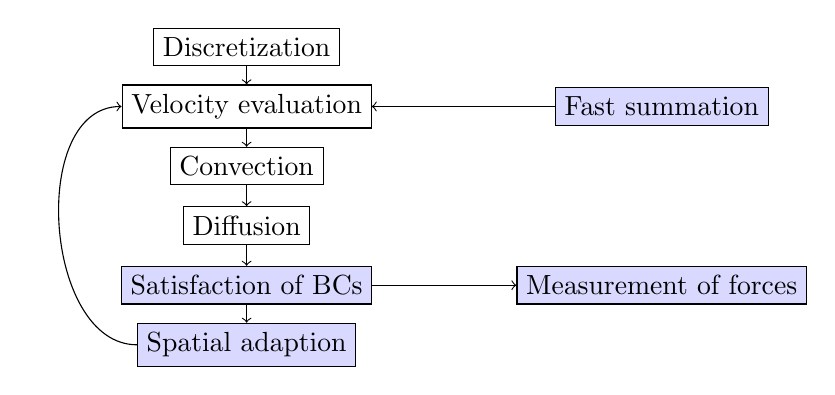
\begin{tikzpicture}[node distance=5ex]
    \node[vm-block]   (disc)                 {Discretization};
    \node[vm-block]   (vel)  [below of=disc] {Velocity evaluation};
    \node[vm-block]   (conv) [below of=vel]  {Convection};
    \node[vm-block]   (diff) [below of=conv] {Diffusion};
    \node[vm-block-o] (bc)   [below of=diff] {Satisfaction of BCs};
    \node[vm-block-o] (spa)  [below of=bc]   {Spatial adaption};
    \node[vm-block-o] (fs)   [right of=vel, node distance=15em] {Fast summation};
    \node[vm-block-o] (mf)   [right of=bc,  node distance=15em] {Measurement of forces};
    \draw[->] (disc) to (vel);
    \draw[->] (vel)  to (conv);
    \draw[->] (conv) to (diff);
    \draw[->] (diff) to (bc);
    \draw[->] (bc)   to (spa);
    \draw[->] (fs)   to (vel);
    \draw[->] (bc)   to (mf);
    \draw[->] (spa.west) to [out=180,in=180] (vel.west);
  \end{tikzpicture}
  \label{fig:vm-blocks}
  \caption{Basic building blocks of a viscous Vortex Method implementation,
    as described in~\cite[\S1.2]{barba04}. Shaded blocks indicate components
    that are not mandatory, but are generally present in modern applications
    of vortex methods.}
\end{figure}

The basic stages of a Vortex Method are those shown in figure~\ref{fig:vm-blocks}.
Each of these stages can be implemented in several different ways.
The discussion below presents some of the alternatives that are possible,
but it is by no means comprehensive.

\subsection{Discretization}
\label{ssec:discretization}

During the discretization stage,
the position and circulation of the particles is set
in order to represent accurately the initial vorticity field.
This includes the choice of the cutoff function~\(\zeta\).

Some classes of methods for particle initialization
described in~\cite[\S2.4]{cottet00} are:
\begin{enumerate}
  \item splitting~\(\supp\vort_0\) in regular cells
    and initializing a particle at the center of each cell;
  \item splitting~\(\supp\vort_0\) in regular cells,
    and for each of them initialize a particle in a random position inside it.
  \item initializing particles randomly in~\(\supp\vort_0\);
\end{enumerate}
If the initial circulation~\(\circulation_p\) is unknown,
it can be set to~\(\circulation_p = \vort_0(\x_p) v_p\),
where \(v_p\) is the volume of the cell
(or an average volume, in the case of random initialization).
Each initialization scheme has different quadrature properties
that determine its accuracy.

Cutoff functions can be constructed in several different ways,
some of which are described in~\cite[\S2.3]{cottet00}.
A customary choice is a Gaussian cutoff:
\begin{equation}
  \zeta_{\sigma k}(\x) =
    \frac{1}{k\pi\sigma^2}
    \exp\left\{\frac{-\norm{\x}^2}{k\sigma^2}\right\},
\end{equation}
which yields an analytical expression for the velocity kernel:
\begin{equation}
  \K_{\sigma k}(\x) =
    \frac{1}{k\pi\norm{\x}^2}
    \left(
      1 - \exp\left\{
        \frac{-\norm{\x}^2}{k\sigma^2}
      \right\}
    \right)
    (-y, x).
\end{equation}
Other choices are possible,
and their accuracy is measured by their moment properties.
A cutoff is said to be of order \(r\) if its \(r\)-th moment is finite
and its moments less than the $r$-th are zero.

\subsection{Velocity evaluation}
\label{ssec:vel-eval}

The evaluation of the velocity is performed by means of
the discrete Biot-Savart law.
The na\"{\i}ve algorithm is
to compute the~\(N\)-term sum in equation~\ref{eq:discrete-biot-savart-law}
for each of the~\(N\) particles,
so velocity evaluation requires~\(O(N^2)\) operations.
Fast summation methods allow to reduce the operation count
by employing a hierarchical domain decomposition and
controlled approximations for the interaction of distant particles.
Two well-known fast summation methods are
Barnes-Hut's~\cite{barnes86} and
the Fast Multipole Method~\cite{greengard87},
which require respectively~\(O(N\log N)\) and~\(O(N)\) operations.

\subsection{Convection}
\label{ssec:convection}

The convection stage consists in moving the particles along the flow.
by integrate equation~\ref{eq:vortex-blob-position-ode}
with a time-stepping algorithm.
The methods of Runge-Kutta and Adams-Bashforth are tipically used.

\subsection{Diffusion}
\label{ssec:diffusion}

\subsection{Satisfaction of boundary conditions}
\label{ssec:bcs}





